\documentclass[11pt,a4paper]{article}

\usepackage[utf8]{inputenc}
\usepackage[T1]{fontenc}
\usepackage[margin=2.5cm]{geometry}
\usepackage{booktabs}
\usepackage{tabularx}
\usepackage{array}
\usepackage{float}
\usepackage{graphicx}
\usepackage{amsmath,amssymb}
\usepackage{newtxtext,newtxmath}
\usepackage{algorithm}
\usepackage{algpseudocode}
\usepackage{caption}
\usepackage{hyperref}
\hypersetup{colorlinks=true, linkcolor=blue, citecolor=blue, urlcolor=blue}

% Supplementary items are cited from the main text as "Table S<n>", "Figure S<n>", "Algorithm S<n>".
\renewcommand{\thetable}{S\arabic{table}}
\renewcommand{\thefigure}{S\arabic{figure}}
\renewcommand{\thealgorithm}{S\arabic{algorithm}}

% Generated by experiments/reporting/export_latex.py -- do not edit.
\providecommand{\R}[1]{\csname rv@#1\endcsname}
\expandafter\def\csname rv@E4.eps_local\endcsname{21}
\expandafter\def\csname rv@E4.epslocal\endcsname{21}
\expandafter\def\csname rv@cost.E0.compute\endcsname{0.09}
\expandafter\def\csname rv@cost.E0.egress\endcsname{0.00}
\expandafter\def\csname rv@cost.E0.egressgb\endcsname{0.0}
\expandafter\def\csname rv@cost.E0.total\endcsname{0.09}
\expandafter\def\csname rv@cost.E0.upgb\endcsname{1.2}
\expandafter\def\csname rv@cost.E1.compute\endcsname{0.00}
\expandafter\def\csname rv@cost.E1.egress\endcsname{2.21}
\expandafter\def\csname rv@cost.E1.egressgb\endcsname{24.6}
\expandafter\def\csname rv@cost.E1.total\endcsname{2.21}
\expandafter\def\csname rv@cost.E1.upgb\endcsname{24.6}
\expandafter\def\csname rv@cost.E2.compute\endcsname{0.00}
\expandafter\def\csname rv@cost.E2.egress\endcsname{2.21}
\expandafter\def\csname rv@cost.E2.egressgb\endcsname{24.6}
\expandafter\def\csname rv@cost.E2.total\endcsname{2.22}
\expandafter\def\csname rv@cost.E2.upgb\endcsname{24.6}
\expandafter\def\csname rv@cost.E3.compute\endcsname{0.19}
\expandafter\def\csname rv@cost.E3.egress\endcsname{2.22}
\expandafter\def\csname rv@cost.E3.egressgb\endcsname{24.6}
\expandafter\def\csname rv@cost.E3.total\endcsname{3.40}
\expandafter\def\csname rv@cost.E3.upgb\endcsname{504.4}
\expandafter\def\csname rv@cost.E3_topk10.compute\endcsname{0.02}
\expandafter\def\csname rv@cost.E3_topk10.egress\endcsname{2.29}
\expandafter\def\csname rv@cost.E3_topk10.egressgb\endcsname{25.4}
\expandafter\def\csname rv@cost.E3_topk10.total\endcsname{3.31}
\expandafter\def\csname rv@cost.E3_topk10.upgb\endcsname{52.5}
\expandafter\def\csname rv@cost.E4.compute\endcsname{0.20}
\expandafter\def\csname rv@cost.E4.egress\endcsname{2.22}
\expandafter\def\csname rv@cost.E4.egressgb\endcsname{24.6}
\expandafter\def\csname rv@cost.E4.total\endcsname{3.41}
\expandafter\def\csname rv@cost.E4.upgb\endcsname{504.4}
\expandafter\def\csname rv@dlg.aggregate_centralnoise_s1.cos\endcsname{\textminus{}0.02}
\expandafter\def\csname rv@dlg.aggregate_centralnoise_s1.mse\endcsname{43.92}
\expandafter\def\csname rv@dlg.aggregate_centralnoise_s1.succ\endcsname{0.00}
\expandafter\def\csname rv@dlg.aggregate_centralnoise_s2.cos\endcsname{\textminus{}0.03}
\expandafter\def\csname rv@dlg.aggregate_centralnoise_s2.mse\endcsname{45.39}
\expandafter\def\csname rv@dlg.aggregate_centralnoise_s2.succ\endcsname{0.00}
\expandafter\def\csname rv@dlg.aggregate_centralnoise_s4.cos\endcsname{\textminus{}0.03}
\expandafter\def\csname rv@dlg.aggregate_centralnoise_s4.mse\endcsname{45.96}
\expandafter\def\csname rv@dlg.aggregate_centralnoise_s4.succ\endcsname{0.00}
\expandafter\def\csname rv@dlg.aggregate_centralnoise_s8.cos\endcsname{\textminus{}0.03}
\expandafter\def\csname rv@dlg.aggregate_centralnoise_s8.mse\endcsname{46.13}
\expandafter\def\csname rv@dlg.aggregate_centralnoise_s8.succ\endcsname{0.00}
\expandafter\def\csname rv@dlg.aggregate_plain.cos\endcsname{0.12}
\expandafter\def\csname rv@dlg.aggregate_plain.mse\endcsname{5.85}
\expandafter\def\csname rv@dlg.aggregate_plain.succ\endcsname{0.06}
\expandafter\def\csname rv@dlg.individual_distnoise_s1.cos\endcsname{\textminus{}0.02}
\expandafter\def\csname rv@dlg.individual_distnoise_s1.mse\endcsname{45.00}
\expandafter\def\csname rv@dlg.individual_distnoise_s1.succ\endcsname{0.00}
\expandafter\def\csname rv@dlg.individual_distnoise_s2.cos\endcsname{\textminus{}0.03}
\expandafter\def\csname rv@dlg.individual_distnoise_s2.mse\endcsname{45.66}
\expandafter\def\csname rv@dlg.individual_distnoise_s2.succ\endcsname{0.00}
\expandafter\def\csname rv@dlg.individual_distnoise_s4.cos\endcsname{\textminus{}0.03}
\expandafter\def\csname rv@dlg.individual_distnoise_s4.mse\endcsname{45.92}
\expandafter\def\csname rv@dlg.individual_distnoise_s4.succ\endcsname{0.00}
\expandafter\def\csname rv@dlg.individual_distnoise_s8.cos\endcsname{\textminus{}0.03}
\expandafter\def\csname rv@dlg.individual_distnoise_s8.mse\endcsname{46.19}
\expandafter\def\csname rv@dlg.individual_distnoise_s8.succ\endcsname{0.00}
\expandafter\def\csname rv@dlg.individual_plain.cos\endcsname{0.87}
\expandafter\def\csname rv@dlg.individual_plain.mse\endcsname{0.47}
\expandafter\def\csname rv@dlg.individual_plain.succ\endcsname{0.96}
\expandafter\def\csname rv@dp.1.eps\endcsname{40.99}
\expandafter\def\csname rv@dp.1.pld\endcsname{7.10}
\expandafter\def\csname rv@dp.2.eps\endcsname{12.10}
\expandafter\def\csname rv@dp.2.pld\endcsname{2.44}
\expandafter\def\csname rv@dp.4.eps\endcsname{4.92}
\expandafter\def\csname rv@dp.4.pld\endcsname{0.99}
\expandafter\def\csname rv@dp.8.eps\endcsname{2.09}
\expandafter\def\csname rv@dp.8.pld\endcsname{0.44}
\expandafter\def\csname rv@ears.E0.d\endcsname{+0.004}
\expandafter\def\csname rv@ears.E0.dhi\endcsname{+0.015}
\expandafter\def\csname rv@ears.E0.dlo\endcsname{\textminus{}0.007}
\expandafter\def\csname rv@ears.E0.n\endcsname{10}
\expandafter\def\csname rv@ears.E0.ndcg\endcsname{0.174}
\expandafter\def\csname rv@ears.E0.ndcghi\endcsname{0.198}
\expandafter\def\csname rv@ears.E0.ndcglo\endcsname{0.150}
\expandafter\def\csname rv@ears.E0.ndcgsd\endcsname{0.033}
\expandafter\def\csname rv@ears.E0.p\endcsname{0.419}
\expandafter\def\csname rv@ears.E0.pw\endcsname{0.492}
\expandafter\def\csname rv@ears.E0.recall\endcsname{0.257}
\expandafter\def\csname rv@ears.E1.n\endcsname{10}
\expandafter\def\csname rv@ears.E1.ndcg\endcsname{0.170}
\expandafter\def\csname rv@ears.E1.ndcghi\endcsname{0.198}
\expandafter\def\csname rv@ears.E1.ndcglo\endcsname{0.142}
\expandafter\def\csname rv@ears.E1.ndcgsd\endcsname{0.039}
\expandafter\def\csname rv@ears.E1.recall\endcsname{0.249}
\expandafter\def\csname rv@ears.E1pop.d\endcsname{\textminus{}0.083}
\expandafter\def\csname rv@ears.E1pop.dhi\endcsname{\textminus{}0.043}
\expandafter\def\csname rv@ears.E1pop.dlo\endcsname{\textminus{}0.123}
\expandafter\def\csname rv@ears.E1untr.d\endcsname{+0.054}
\expandafter\def\csname rv@ears.E1untr.dhi\endcsname{+0.103}
\expandafter\def\csname rv@ears.E1untr.dlo\endcsname{+0.006}
\expandafter\def\csname rv@ears.E1untr.p\endcsname{0.033}
\expandafter\def\csname rv@ears.E2_s1.d\endcsname{+0.039}
\expandafter\def\csname rv@ears.E2_s1.dhi\endcsname{+0.102}
\expandafter\def\csname rv@ears.E2_s1.dlo\endcsname{\textminus{}0.024}
\expandafter\def\csname rv@ears.E2_s1.eps\endcsname{41.0}
\expandafter\def\csname rv@ears.E2_s1.n\endcsname{10}
\expandafter\def\csname rv@ears.E2_s1.ndcg\endcsname{0.209}
\expandafter\def\csname rv@ears.E2_s1.ndcghi\endcsname{0.290}
\expandafter\def\csname rv@ears.E2_s1.ndcglo\endcsname{0.128}
\expandafter\def\csname rv@ears.E2_s1.ndcgsd\endcsname{0.113}
\expandafter\def\csname rv@ears.E2_s1.p\endcsname{0.197}
\expandafter\def\csname rv@ears.E2_s1.pw\endcsname{0.160}
\expandafter\def\csname rv@ears.E2_s1.recall\endcsname{0.290}
\expandafter\def\csname rv@ears.E2_s2.d\endcsname{+0.021}
\expandafter\def\csname rv@ears.E2_s2.dhi\endcsname{+0.112}
\expandafter\def\csname rv@ears.E2_s2.dlo\endcsname{\textminus{}0.069}
\expandafter\def\csname rv@ears.E2_s2.eps\endcsname{12.1}
\expandafter\def\csname rv@ears.E2_s2.n\endcsname{10}
\expandafter\def\csname rv@ears.E2_s2.ndcg\endcsname{0.192}
\expandafter\def\csname rv@ears.E2_s2.ndcghi\endcsname{0.300}
\expandafter\def\csname rv@ears.E2_s2.ndcglo\endcsname{0.083}
\expandafter\def\csname rv@ears.E2_s2.ndcgsd\endcsname{0.152}
\expandafter\def\csname rv@ears.E2_s2.p\endcsname{0.606}
\expandafter\def\csname rv@ears.E2_s2.pw\endcsname{0.625}
\expandafter\def\csname rv@ears.E2_s2.recall\endcsname{0.257}
\expandafter\def\csname rv@ears.E2_s4.d\endcsname{+0.030}
\expandafter\def\csname rv@ears.E2_s4.dhi\endcsname{+0.138}
\expandafter\def\csname rv@ears.E2_s4.dlo\endcsname{\textminus{}0.077}
\expandafter\def\csname rv@ears.E2_s4.eps\endcsname{4.9}
\expandafter\def\csname rv@ears.E2_s4.n\endcsname{10}
\expandafter\def\csname rv@ears.E2_s4.ndcg\endcsname{0.200}
\expandafter\def\csname rv@ears.E2_s4.ndcghi\endcsname{0.319}
\expandafter\def\csname rv@ears.E2_s4.ndcglo\endcsname{0.082}
\expandafter\def\csname rv@ears.E2_s4.ndcgsd\endcsname{0.166}
\expandafter\def\csname rv@ears.E2_s4.p\endcsname{0.541}
\expandafter\def\csname rv@ears.E2_s4.pw\endcsname{1.000}
\expandafter\def\csname rv@ears.E2_s4.recall\endcsname{0.258}
\expandafter\def\csname rv@ears.E2_s8.d\endcsname{+0.060}
\expandafter\def\csname rv@ears.E2_s8.dhi\endcsname{+0.171}
\expandafter\def\csname rv@ears.E2_s8.dlo\endcsname{\textminus{}0.051}
\expandafter\def\csname rv@ears.E2_s8.eps\endcsname{2.1}
\expandafter\def\csname rv@ears.E2_s8.n\endcsname{10}
\expandafter\def\csname rv@ears.E2_s8.ndcg\endcsname{0.230}
\expandafter\def\csname rv@ears.E2_s8.ndcghi\endcsname{0.357}
\expandafter\def\csname rv@ears.E2_s8.ndcglo\endcsname{0.104}
\expandafter\def\csname rv@ears.E2_s8.ndcgsd\endcsname{0.177}
\expandafter\def\csname rv@ears.E2_s8.p\endcsname{0.253}
\expandafter\def\csname rv@ears.E2_s8.pw\endcsname{0.625}
\expandafter\def\csname rv@ears.E2_s8.recall\endcsname{0.270}
\expandafter\def\csname rv@ears.E3.ci90hi\endcsname{+0.0009}
\expandafter\def\csname rv@ears.E3.ci90lo\endcsname{\textminus{}0.0004}
\expandafter\def\csname rv@ears.E3.d\endcsname{+0.0003}
\expandafter\def\csname rv@ears.E3.dhi\endcsname{+0.001}
\expandafter\def\csname rv@ears.E3.dlo\endcsname{\textminus{}0.001}
\expandafter\def\csname rv@ears.E3.equiv\endcsname{yes}
\expandafter\def\csname rv@ears.E3.mde\endcsname{0.0011}
\expandafter\def\csname rv@ears.E3.n\endcsname{10}
\expandafter\def\csname rv@ears.E3.ndcg\endcsname{0.170}
\expandafter\def\csname rv@ears.E3.ndcghi\endcsname{0.198}
\expandafter\def\csname rv@ears.E3.ndcglo\endcsname{0.143}
\expandafter\def\csname rv@ears.E3.ndcgsd\endcsname{0.038}
\expandafter\def\csname rv@ears.E3.p\endcsname{0.465}
\expandafter\def\csname rv@ears.E3.ptost\endcsname{$<$0.001}
\expandafter\def\csname rv@ears.E3.pw\endcsname{0.625}
\expandafter\def\csname rv@ears.E3.recall\endcsname{0.249}
\expandafter\def\csname rv@ears.E3.sdd\endcsname{0.0011}
\expandafter\def\csname rv@ears.E4.d\endcsname{+0.105}
\expandafter\def\csname rv@ears.E4.dhi\endcsname{+0.257}
\expandafter\def\csname rv@ears.E4.dlo\endcsname{\textminus{}0.047}
\expandafter\def\csname rv@ears.E4.eps\endcsname{4.9}
\expandafter\def\csname rv@ears.E4.n\endcsname{10}
\expandafter\def\csname rv@ears.E4.ndcg\endcsname{0.275}
\expandafter\def\csname rv@ears.E4.ndcghi\endcsname{0.421}
\expandafter\def\csname rv@ears.E4.ndcglo\endcsname{0.129}
\expandafter\def\csname rv@ears.E4.ndcgsd\endcsname{0.204}
\expandafter\def\csname rv@ears.E4.p\endcsname{0.154}
\expandafter\def\csname rv@ears.E4.pw\endcsname{0.322}
\expandafter\def\csname rv@ears.E4.recall\endcsname{0.324}
\expandafter\def\csname rv@ears.cutoff\endcsname{2026-03-08}
\expandafter\def\csname rv@ears.noise.e4.d\endcsname{\textminus{}0.002}
\expandafter\def\csname rv@ears.noise.e4.dhi\endcsname{+0.141}
\expandafter\def\csname rv@ears.noise.e4.dlo\endcsname{\textminus{}0.145}
\expandafter\def\csname rv@ears.noise.s1.d\endcsname{+0.045}
\expandafter\def\csname rv@ears.noise.s1.dhi\endcsname{+0.133}
\expandafter\def\csname rv@ears.noise.s1.dlo\endcsname{\textminus{}0.043}
\expandafter\def\csname rv@ears.noise.s1.ndcg\endcsname{0.164}
\expandafter\def\csname rv@ears.noise.s1.norm\endcsname{153}
\expandafter\def\csname rv@ears.noise.s1.p\endcsname{0.279}
\expandafter\def\csname rv@ears.noise.s2.d\endcsname{\textminus{}0.040}
\expandafter\def\csname rv@ears.noise.s2.dhi\endcsname{+0.083}
\expandafter\def\csname rv@ears.noise.s2.dlo\endcsname{\textminus{}0.164}
\expandafter\def\csname rv@ears.noise.s2.ndcg\endcsname{0.232}
\expandafter\def\csname rv@ears.noise.s2.norm\endcsname{306}
\expandafter\def\csname rv@ears.noise.s2.p\endcsname{0.479}
\expandafter\def\csname rv@ears.noise.s4.d\endcsname{\textminus{}0.077}
\expandafter\def\csname rv@ears.noise.s4.dhi\endcsname{+0.052}
\expandafter\def\csname rv@ears.noise.s4.dlo\endcsname{\textminus{}0.205}
\expandafter\def\csname rv@ears.noise.s4.ndcg\endcsname{0.277}
\expandafter\def\csname rv@ears.noise.s4.norm\endcsname{613}
\expandafter\def\csname rv@ears.noise.s4.p\endcsname{0.211}
\expandafter\def\csname rv@ears.noise.s8.d\endcsname{\textminus{}0.081}
\expandafter\def\csname rv@ears.noise.s8.dhi\endcsname{+0.063}
\expandafter\def\csname rv@ears.noise.s8.dlo\endcsname{\textminus{}0.225}
\expandafter\def\csname rv@ears.noise.s8.ndcg\endcsname{0.311}
\expandafter\def\csname rv@ears.noise.s8.norm\endcsname{1,226}
\expandafter\def\csname rv@ears.noise.s8.p\endcsname{0.235}
\expandafter\def\csname rv@ears.popularity.ndcg\endcsname{0.253}
\expandafter\def\csname rv@ears.pos.max\endcsname{144}
\expandafter\def\csname rv@ears.pos.min\endcsname{108}
\expandafter\def\csname rv@ears.random.ndcg\endcsname{0.110}
\expandafter\def\csname rv@ears.untrained.ndcg\endcsname{0.116}
\expandafter\def\csname rv@mcda.b2b.first\endcsname{E3}
\expandafter\def\csname rv@mcda.b2b.oat\endcsname{yes}
\expandafter\def\csname rv@mcda.b2b.pfirst\endcsname{0.68}
\expandafter\def\csname rv@mcda.reg.first\endcsname{E3}
\expandafter\def\csname rv@mcda.reg.oat\endcsname{yes}
\expandafter\def\csname rv@mcda.reg.pfirst\endcsname{0.55}
\expandafter\def\csname rv@mcda.ret.first\endcsname{E0}
\expandafter\def\csname rv@mcda.ret.oat\endcsname{yes}
\expandafter\def\csname rv@mcda.ret.pfirst\endcsname{0.86}
\expandafter\def\csname rv@mia.E0.cauc\endcsname{0.49}
\expandafter\def\csname rv@mia.E0.csig\endcsname{0/10}
\expandafter\def\csname rv@mia.E0.rauc\endcsname{0.498}
\expandafter\def\csname rv@mia.E0.rlow\endcsname{1/10}
\expandafter\def\csname rv@mia.E0.rsig\endcsname{1/10}
\expandafter\def\csname rv@mia.E1.cauc\endcsname{0.49}
\expandafter\def\csname rv@mia.E1.csig\endcsname{0/10}
\expandafter\def\csname rv@mia.E1.rauc\endcsname{0.499}
\expandafter\def\csname rv@mia.E1.rlow\endcsname{1/10}
\expandafter\def\csname rv@mia.E1.rsig\endcsname{1/10}
\expandafter\def\csname rv@mia.E2_s1.cauc\endcsname{0.51}
\expandafter\def\csname rv@mia.E2_s1.csig\endcsname{0/10}
\expandafter\def\csname rv@mia.E2_s1.rauc\endcsname{0.494}
\expandafter\def\csname rv@mia.E2_s1.rlow\endcsname{1/10}
\expandafter\def\csname rv@mia.E2_s1.rsig\endcsname{1/10}
\expandafter\def\csname rv@mia.E2_s2.cauc\endcsname{0.49}
\expandafter\def\csname rv@mia.E2_s2.csig\endcsname{1/10}
\expandafter\def\csname rv@mia.E2_s2.rauc\endcsname{0.498}
\expandafter\def\csname rv@mia.E2_s2.rlow\endcsname{1/10}
\expandafter\def\csname rv@mia.E2_s2.rsig\endcsname{1/10}
\expandafter\def\csname rv@mia.E2_s4.cauc\endcsname{0.49}
\expandafter\def\csname rv@mia.E2_s4.csig\endcsname{1/10}
\expandafter\def\csname rv@mia.E2_s4.rauc\endcsname{0.499}
\expandafter\def\csname rv@mia.E2_s4.rlow\endcsname{1/10}
\expandafter\def\csname rv@mia.E2_s4.rsig\endcsname{1/10}
\expandafter\def\csname rv@mia.E2_s8.cauc\endcsname{0.48}
\expandafter\def\csname rv@mia.E2_s8.csig\endcsname{0/10}
\expandafter\def\csname rv@mia.E2_s8.rauc\endcsname{0.497}
\expandafter\def\csname rv@mia.E2_s8.rlow\endcsname{0/10}
\expandafter\def\csname rv@mia.E2_s8.rsig\endcsname{0/10}
\expandafter\def\csname rv@mia.E3.cauc\endcsname{0.49}
\expandafter\def\csname rv@mia.E3.csig\endcsname{0/10}
\expandafter\def\csname rv@mia.E3.rauc\endcsname{0.499}
\expandafter\def\csname rv@mia.E3.rlow\endcsname{1/10}
\expandafter\def\csname rv@mia.E3.rsig\endcsname{1/10}
\expandafter\def\csname rv@mia.E4.cauc\endcsname{0.52}
\expandafter\def\csname rv@mia.E4.csig\endcsname{2/10}
\expandafter\def\csname rv@mia.E4.rauc\endcsname{0.500}
\expandafter\def\csname rv@mia.E4.rlow\endcsname{0/10}
\expandafter\def\csname rv@mia.E4.rsig\endcsname{0/10}
\expandafter\def\csname rv@miaml.E0.cauc\endcsname{0.47}
\expandafter\def\csname rv@miaml.E0.rauc\endcsname{0.506}
\expandafter\def\csname rv@miaml.E1.cauc\endcsname{0.47}
\expandafter\def\csname rv@miaml.E1.rauc\endcsname{0.506}
\expandafter\def\csname rv@miaml.E2_s1.cauc\endcsname{0.47}
\expandafter\def\csname rv@miaml.E2_s1.rauc\endcsname{0.500}
\expandafter\def\csname rv@miaml.E2_s2.cauc\endcsname{0.49}
\expandafter\def\csname rv@miaml.E2_s2.rauc\endcsname{0.497}
\expandafter\def\csname rv@miaml.E2_s4.cauc\endcsname{0.52}
\expandafter\def\csname rv@miaml.E2_s4.rauc\endcsname{0.501}
\expandafter\def\csname rv@miaml.E2_s8.cauc\endcsname{0.56}
\expandafter\def\csname rv@miaml.E2_s8.rauc\endcsname{0.503}
\expandafter\def\csname rv@miaml.E3.cauc\endcsname{0.47}
\expandafter\def\csname rv@miaml.E3.rauc\endcsname{0.506}
\expandafter\def\csname rv@miaml.E4.cauc\endcsname{0.49}
\expandafter\def\csname rv@miaml.E4.rauc\endcsname{0.504}
\expandafter\def\csname rv@movielens.E0.d\endcsname{+0.004}
\expandafter\def\csname rv@movielens.E0.dhi\endcsname{+0.014}
\expandafter\def\csname rv@movielens.E0.dlo\endcsname{\textminus{}0.006}
\expandafter\def\csname rv@movielens.E0.n\endcsname{10}
\expandafter\def\csname rv@movielens.E0.ndcg\endcsname{0.260}
\expandafter\def\csname rv@movielens.E0.ndcghi\endcsname{0.279}
\expandafter\def\csname rv@movielens.E0.ndcglo\endcsname{0.242}
\expandafter\def\csname rv@movielens.E0.ndcgsd\endcsname{0.026}
\expandafter\def\csname rv@movielens.E0.p\endcsname{0.368}
\expandafter\def\csname rv@movielens.E0.pw\endcsname{0.232}
\expandafter\def\csname rv@movielens.E0.recall\endcsname{0.202}
\expandafter\def\csname rv@movielens.E1.n\endcsname{10}
\expandafter\def\csname rv@movielens.E1.ndcg\endcsname{0.256}
\expandafter\def\csname rv@movielens.E1.ndcghi\endcsname{0.277}
\expandafter\def\csname rv@movielens.E1.ndcglo\endcsname{0.236}
\expandafter\def\csname rv@movielens.E1.ndcgsd\endcsname{0.029}
\expandafter\def\csname rv@movielens.E1.recall\endcsname{0.199}
\expandafter\def\csname rv@movielens.E1pop.d\endcsname{\textminus{}0.307}
\expandafter\def\csname rv@movielens.E1pop.dhi\endcsname{\textminus{}0.288}
\expandafter\def\csname rv@movielens.E1pop.dlo\endcsname{\textminus{}0.326}
\expandafter\def\csname rv@movielens.E1untr.d\endcsname{+0.052}
\expandafter\def\csname rv@movielens.E1untr.dhi\endcsname{+0.077}
\expandafter\def\csname rv@movielens.E1untr.dlo\endcsname{+0.026}
\expandafter\def\csname rv@movielens.E1untr.p\endcsname{0.001}
\expandafter\def\csname rv@movielens.E2_s1.d\endcsname{\textminus{}0.008}
\expandafter\def\csname rv@movielens.E2_s1.dhi\endcsname{+0.078}
\expandafter\def\csname rv@movielens.E2_s1.dlo\endcsname{\textminus{}0.094}
\expandafter\def\csname rv@movielens.E2_s1.eps\endcsname{41.0}
\expandafter\def\csname rv@movielens.E2_s1.n\endcsname{10}
\expandafter\def\csname rv@movielens.E2_s1.ndcg\endcsname{0.248}
\expandafter\def\csname rv@movielens.E2_s1.ndcghi\endcsname{0.326}
\expandafter\def\csname rv@movielens.E2_s1.ndcglo\endcsname{0.170}
\expandafter\def\csname rv@movielens.E2_s1.ndcgsd\endcsname{0.109}
\expandafter\def\csname rv@movielens.E2_s1.p\endcsname{0.833}
\expandafter\def\csname rv@movielens.E2_s1.pw\endcsname{0.432}
\expandafter\def\csname rv@movielens.E2_s1.recall\endcsname{0.191}
\expandafter\def\csname rv@movielens.E2_s2.d\endcsname{+0.030}
\expandafter\def\csname rv@movielens.E2_s2.dhi\endcsname{+0.114}
\expandafter\def\csname rv@movielens.E2_s2.dlo\endcsname{\textminus{}0.053}
\expandafter\def\csname rv@movielens.E2_s2.eps\endcsname{12.1}
\expandafter\def\csname rv@movielens.E2_s2.n\endcsname{10}
\expandafter\def\csname rv@movielens.E2_s2.ndcg\endcsname{0.287}
\expandafter\def\csname rv@movielens.E2_s2.ndcghi\endcsname{0.366}
\expandafter\def\csname rv@movielens.E2_s2.ndcglo\endcsname{0.208}
\expandafter\def\csname rv@movielens.E2_s2.ndcgsd\endcsname{0.111}
\expandafter\def\csname rv@movielens.E2_s2.p\endcsname{0.432}
\expandafter\def\csname rv@movielens.E2_s2.pw\endcsname{1.000}
\expandafter\def\csname rv@movielens.E2_s2.recall\endcsname{0.214}
\expandafter\def\csname rv@movielens.E2_s4.d\endcsname{+0.059}
\expandafter\def\csname rv@movielens.E2_s4.dhi\endcsname{+0.160}
\expandafter\def\csname rv@movielens.E2_s4.dlo\endcsname{\textminus{}0.042}
\expandafter\def\csname rv@movielens.E2_s4.eps\endcsname{4.9}
\expandafter\def\csname rv@movielens.E2_s4.n\endcsname{10}
\expandafter\def\csname rv@movielens.E2_s4.ndcg\endcsname{0.315}
\expandafter\def\csname rv@movielens.E2_s4.ndcghi\endcsname{0.419}
\expandafter\def\csname rv@movielens.E2_s4.ndcglo\endcsname{0.211}
\expandafter\def\csname rv@movielens.E2_s4.ndcgsd\endcsname{0.145}
\expandafter\def\csname rv@movielens.E2_s4.p\endcsname{0.221}
\expandafter\def\csname rv@movielens.E2_s4.pw\endcsname{0.232}
\expandafter\def\csname rv@movielens.E2_s4.recall\endcsname{0.228}
\expandafter\def\csname rv@movielens.E2_s8.d\endcsname{+0.070}
\expandafter\def\csname rv@movielens.E2_s8.dhi\endcsname{+0.173}
\expandafter\def\csname rv@movielens.E2_s8.dlo\endcsname{\textminus{}0.032}
\expandafter\def\csname rv@movielens.E2_s8.eps\endcsname{2.1}
\expandafter\def\csname rv@movielens.E2_s8.n\endcsname{10}
\expandafter\def\csname rv@movielens.E2_s8.ndcg\endcsname{0.327}
\expandafter\def\csname rv@movielens.E2_s8.ndcghi\endcsname{0.434}
\expandafter\def\csname rv@movielens.E2_s8.ndcglo\endcsname{0.220}
\expandafter\def\csname rv@movielens.E2_s8.ndcgsd\endcsname{0.150}
\expandafter\def\csname rv@movielens.E2_s8.p\endcsname{0.155}
\expandafter\def\csname rv@movielens.E2_s8.pw\endcsname{0.160}
\expandafter\def\csname rv@movielens.E2_s8.recall\endcsname{0.231}
\expandafter\def\csname rv@movielens.E3.ci90hi\endcsname{+0.0037}
\expandafter\def\csname rv@movielens.E3.ci90lo\endcsname{\textminus{}0.0012}
\expandafter\def\csname rv@movielens.E3.d\endcsname{+0.0013}
\expandafter\def\csname rv@movielens.E3.dhi\endcsname{+0.004}
\expandafter\def\csname rv@movielens.E3.dlo\endcsname{\textminus{}0.002}
\expandafter\def\csname rv@movielens.E3.equiv\endcsname{yes}
\expandafter\def\csname rv@movielens.E3.mde\endcsname{0.0042}
\expandafter\def\csname rv@movielens.E3.n\endcsname{10}
\expandafter\def\csname rv@movielens.E3.ndcg\endcsname{0.258}
\expandafter\def\csname rv@movielens.E3.ndcghi\endcsname{0.278}
\expandafter\def\csname rv@movielens.E3.ndcglo\endcsname{0.237}
\expandafter\def\csname rv@movielens.E3.ndcgsd\endcsname{0.028}
\expandafter\def\csname rv@movielens.E3.p\endcsname{0.363}
\expandafter\def\csname rv@movielens.E3.ptost\endcsname{$<$0.001}
\expandafter\def\csname rv@movielens.E3.pw\endcsname{0.193}
\expandafter\def\csname rv@movielens.E3.recall\endcsname{0.199}
\expandafter\def\csname rv@movielens.E3.sdd\endcsname{0.0042}
\expandafter\def\csname rv@movielens.E4.d\endcsname{+0.056}
\expandafter\def\csname rv@movielens.E4.dhi\endcsname{+0.140}
\expandafter\def\csname rv@movielens.E4.dlo\endcsname{\textminus{}0.028}
\expandafter\def\csname rv@movielens.E4.eps\endcsname{4.9}
\expandafter\def\csname rv@movielens.E4.n\endcsname{10}
\expandafter\def\csname rv@movielens.E4.ndcg\endcsname{0.312}
\expandafter\def\csname rv@movielens.E4.ndcghi\endcsname{0.400}
\expandafter\def\csname rv@movielens.E4.ndcglo\endcsname{0.224}
\expandafter\def\csname rv@movielens.E4.ndcgsd\endcsname{0.123}
\expandafter\def\csname rv@movielens.E4.p\endcsname{0.169}
\expandafter\def\csname rv@movielens.E4.pw\endcsname{0.557}
\expandafter\def\csname rv@movielens.E4.recall\endcsname{0.228}
\expandafter\def\csname rv@movielens.cutoff\endcsname{1998-03-08}
\expandafter\def\csname rv@movielens.noise.e4.d\endcsname{+0.017}
\expandafter\def\csname rv@movielens.noise.e4.dhi\endcsname{+0.102}
\expandafter\def\csname rv@movielens.noise.e4.dlo\endcsname{\textminus{}0.069}
\expandafter\def\csname rv@movielens.noise.s1.d\endcsname{+0.029}
\expandafter\def\csname rv@movielens.noise.s1.dhi\endcsname{+0.114}
\expandafter\def\csname rv@movielens.noise.s1.dlo\endcsname{\textminus{}0.056}
\expandafter\def\csname rv@movielens.noise.s1.ndcg\endcsname{0.219}
\expandafter\def\csname rv@movielens.noise.s1.norm\endcsname{153}
\expandafter\def\csname rv@movielens.noise.s1.p\endcsname{0.464}
\expandafter\def\csname rv@movielens.noise.s2.d\endcsname{+0.022}
\expandafter\def\csname rv@movielens.noise.s2.dhi\endcsname{+0.099}
\expandafter\def\csname rv@movielens.noise.s2.dlo\endcsname{\textminus{}0.054}
\expandafter\def\csname rv@movielens.noise.s2.ndcg\endcsname{0.264}
\expandafter\def\csname rv@movielens.noise.s2.norm\endcsname{306}
\expandafter\def\csname rv@movielens.noise.s2.p\endcsname{0.525}
\expandafter\def\csname rv@movielens.noise.s4.d\endcsname{+0.020}
\expandafter\def\csname rv@movielens.noise.s4.dhi\endcsname{+0.122}
\expandafter\def\csname rv@movielens.noise.s4.dlo\endcsname{\textminus{}0.082}
\expandafter\def\csname rv@movielens.noise.s4.ndcg\endcsname{0.295}
\expandafter\def\csname rv@movielens.noise.s4.norm\endcsname{613}
\expandafter\def\csname rv@movielens.noise.s4.p\endcsname{0.670}
\expandafter\def\csname rv@movielens.noise.s8.d\endcsname{+0.024}
\expandafter\def\csname rv@movielens.noise.s8.dhi\endcsname{+0.127}
\expandafter\def\csname rv@movielens.noise.s8.dlo\endcsname{\textminus{}0.079}
\expandafter\def\csname rv@movielens.noise.s8.ndcg\endcsname{0.303}
\expandafter\def\csname rv@movielens.noise.s8.norm\endcsname{1,226}
\expandafter\def\csname rv@movielens.noise.s8.p\endcsname{0.613}
\expandafter\def\csname rv@movielens.popularity.ndcg\endcsname{0.563}
\expandafter\def\csname rv@movielens.pos.max\endcsname{1{,}097}
\expandafter\def\csname rv@movielens.pos.min\endcsname{630}
\expandafter\def\csname rv@movielens.random.ndcg\endcsname{0.206}
\expandafter\def\csname rv@movielens.untrained.ndcg\endcsname{0.205}
\expandafter\def\csname rv@nparams\endcsname{586{,}700}
\expandafter\def\csname rv@oh.E1.agg\endcsname{0.04}
\expandafter\def\csname rv@oh.E1.ctx\endcsname{0.0}
\expandafter\def\csname rv@oh.E1.dec\endcsname{0.00}
\expandafter\def\csname rv@oh.E1.down\endcsname{167.9}
\expandafter\def\csname rv@oh.E1.enc\endcsname{0.00}
\expandafter\def\csname rv@oh.E1.up\endcsname{167.9}
\expandafter\def\csname rv@oh.E2_s4.agg\endcsname{0.17}
\expandafter\def\csname rv@oh.E2_s4.ctx\endcsname{0.0}
\expandafter\def\csname rv@oh.E2_s4.dec\endcsname{0.00}
\expandafter\def\csname rv@oh.E2_s4.down\endcsname{167.9}
\expandafter\def\csname rv@oh.E2_s4.enc\endcsname{0.00}
\expandafter\def\csname rv@oh.E2_s4.up\endcsname{167.9}
\expandafter\def\csname rv@oh.E3.agg\endcsname{11.36}
\expandafter\def\csname rv@oh.E3.ctx\endcsname{9.0}
\expandafter\def\csname rv@oh.E3.dec\endcsname{1.75}
\expandafter\def\csname rv@oh.E3.down\endcsname{167.9}
\expandafter\def\csname rv@oh.E3.enc\endcsname{33.09}
\expandafter\def\csname rv@oh.E3.up\endcsname{3,443.1}
\expandafter\def\csname rv@oh.E4.agg\endcsname{12.08}
\expandafter\def\csname rv@oh.E4.ctx\endcsname{9.0}
\expandafter\def\csname rv@oh.E4.dec\endcsname{1.85}
\expandafter\def\csname rv@oh.E4.down\endcsname{167.9}
\expandafter\def\csname rv@oh.E4.enc\endcsname{33.70}
\expandafter\def\csname rv@oh.E4.up\endcsname{3,443.1}
\expandafter\def\csname rv@oh.ratio\endcsname{20.5}
\expandafter\def\csname rv@power.0.005\endcsname{1.00}
\expandafter\def\csname rv@power.0.01\endcsname{0.80}
\expandafter\def\csname rv@power.0.02\endcsname{0.29}
\expandafter\def\csname rv@tk.05.agg\endcsname{0.70}
\expandafter\def\csname rv@tk.05.he.d\endcsname{+0.001}
\expandafter\def\csname rv@tk.05.he.dhi\endcsname{+0.024}
\expandafter\def\csname rv@tk.05.he.dlo\endcsname{\textminus{}0.021}
\expandafter\def\csname rv@tk.05.hp.d\endcsname{+0.019}
\expandafter\def\csname rv@tk.05.hp.dhi\endcsname{+0.046}
\expandafter\def\csname rv@tk.05.hp.dlo\endcsname{\textminus{}0.008}
\expandafter\def\csname rv@tk.05.mask\endcsname{5.25}
\expandafter\def\csname rv@tk.05.ndcg\endcsname{0.172}
\expandafter\def\csname rv@tk.05.pl.d\endcsname{\textminus{}0.017}
\expandafter\def\csname rv@tk.05.pl.dhi\endcsname{+0.017}
\expandafter\def\csname rv@tk.05.pl.dlo\endcsname{\textminus{}0.051}
\expandafter\def\csname rv@tk.05.plainndcg\endcsname{0.153}
\expandafter\def\csname rv@tk.05.plainup\endcsname{16.8}
\expandafter\def\csname rv@tk.05.red\endcsname{94.4}
\expandafter\def\csname rv@tk.05.up\endcsname{191.3}
\expandafter\def\csname rv@tk.10.agg\endcsname{1.32}
\expandafter\def\csname rv@tk.10.he.d\endcsname{+0.003}
\expandafter\def\csname rv@tk.10.he.dhi\endcsname{+0.021}
\expandafter\def\csname rv@tk.10.he.dlo\endcsname{\textminus{}0.014}
\expandafter\def\csname rv@tk.10.hp.d\endcsname{+0.010}
\expandafter\def\csname rv@tk.10.hp.dhi\endcsname{+0.037}
\expandafter\def\csname rv@tk.10.hp.dlo\endcsname{\textminus{}0.017}
\expandafter\def\csname rv@tk.10.mask\endcsname{5.25}
\expandafter\def\csname rv@tk.10.ndcg\endcsname{0.174}
\expandafter\def\csname rv@tk.10.pl.d\endcsname{\textminus{}0.006}
\expandafter\def\csname rv@tk.10.pl.dhi\endcsname{+0.021}
\expandafter\def\csname rv@tk.10.pl.dlo\endcsname{\textminus{}0.034}
\expandafter\def\csname rv@tk.10.plainndcg\endcsname{0.164}
\expandafter\def\csname rv@tk.10.plainup\endcsname{33.6}
\expandafter\def\csname rv@tk.10.red\endcsname{89.6}
\expandafter\def\csname rv@tk.10.up\endcsname{358.7}
\expandafter\def\csname rv@tk.20.agg\endcsname{2.57}
\expandafter\def\csname rv@tk.20.he.d\endcsname{\textminus{}0.002}
\expandafter\def\csname rv@tk.20.he.dhi\endcsname{+0.010}
\expandafter\def\csname rv@tk.20.he.dlo\endcsname{\textminus{}0.014}
\expandafter\def\csname rv@tk.20.hp.d\endcsname{+0.002}
\expandafter\def\csname rv@tk.20.hp.dhi\endcsname{+0.007}
\expandafter\def\csname rv@tk.20.hp.dlo\endcsname{\textminus{}0.003}
\expandafter\def\csname rv@tk.20.mask\endcsname{5.25}
\expandafter\def\csname rv@tk.20.ndcg\endcsname{0.168}
\expandafter\def\csname rv@tk.20.pl.d\endcsname{\textminus{}0.004}
\expandafter\def\csname rv@tk.20.pl.dhi\endcsname{+0.004}
\expandafter\def\csname rv@tk.20.pl.dlo\endcsname{\textminus{}0.012}
\expandafter\def\csname rv@tk.20.plainndcg\endcsname{0.166}
\expandafter\def\csname rv@tk.20.plainup\endcsname{67.1}
\expandafter\def\csname rv@tk.20.red\endcsname{79.9}
\expandafter\def\csname rv@tk.20.up\endcsname{693.4}
\expandafter\def\csname rv@tk.50.agg\endcsname{6.29}
\expandafter\def\csname rv@tk.50.he.d\endcsname{\textminus{}0.004}
\expandafter\def\csname rv@tk.50.he.dhi\endcsname{+0.002}
\expandafter\def\csname rv@tk.50.he.dlo\endcsname{\textminus{}0.010}
\expandafter\def\csname rv@tk.50.hp.d\endcsname{\textminus{}0.006}
\expandafter\def\csname rv@tk.50.hp.dhi\endcsname{\textminus{}0.002}
\expandafter\def\csname rv@tk.50.hp.dlo\endcsname{\textminus{}0.011}
\expandafter\def\csname rv@tk.50.mask\endcsname{5.25}
\expandafter\def\csname rv@tk.50.ndcg\endcsname{0.167}
\expandafter\def\csname rv@tk.50.pl.d\endcsname{+0.003}
\expandafter\def\csname rv@tk.50.pl.dhi\endcsname{+0.005}
\expandafter\def\csname rv@tk.50.pl.dlo\endcsname{0.000}
\expandafter\def\csname rv@tk.50.plainndcg\endcsname{0.173}
\expandafter\def\csname rv@tk.50.plainup\endcsname{167.9}
\expandafter\def\csname rv@tk.50.red\endcsname{50.0}
\expandafter\def\csname rv@tk.50.up\endcsname{1,721.5}
\expandafter\def\csname rv@xai.E0.coal\endcsname{200}
\expandafter\def\csname rv@xai.E0.gap_cond\endcsname{0.39}
\expandafter\def\csname rv@xai.E0.gap_marg\endcsname{0.36}
\expandafter\def\csname rv@xai.E0.lime_d_s\endcsname{0.16}
\expandafter\def\csname rv@xai.E0.lime_gap_cond\endcsname{0.37}
\expandafter\def\csname rv@xai.E0.lime_m_rows\endcsname{4,001}
\expandafter\def\csname rv@xai.E0.lime_m_s\endcsname{0.12}
\expandafter\def\csname rv@xai.E0.lime_m_us_row\endcsname{30.61}
\expandafter\def\csname rv@xai.E0.nn_conditional_k10\endcsname{3.32}
\expandafter\def\csname rv@xai.E0.nn_conditional_k10_inc\endcsname{\textminus{}0.16}
\expandafter\def\csname rv@xai.E0.nn_conditional_k3\endcsname{3.48}
\expandafter\def\csname rv@xai.E0.nn_inst\endcsname{3.64}
\expandafter\def\csname rv@xai.E0.nn_marginal_k10\endcsname{4.40}
\expandafter\def\csname rv@xai.E0.nn_marginal_k10_inc\endcsname{0.50}
\expandafter\def\csname rv@xai.E0.nn_marginal_k3\endcsname{3.73}
\expandafter\def\csname rv@xai.E0.nn_real\endcsname{2.29}
\expandafter\def\csname rv@xai.E0.shap_calls\endcsname{2.00}
\expandafter\def\csname rv@xai.E0.shap_lime_rho\endcsname{0.46}
\expandafter\def\csname rv@xai.E0.shap_rows\endcsname{4,001}
\expandafter\def\csname rv@xai.E0.shap_s\endcsname{0.11}
\expandafter\def\csname rv@xai.E0.shap_us_row\endcsname{28.69}
\expandafter\def\csname rv@xai.E0.stab_rho\endcsname{0.82}
\expandafter\def\csname rv@xai.E1.agree_rho\endcsname{0.86}
\expandafter\def\csname rv@xai.E1.agree_top5\endcsname{0.78}
\expandafter\def\csname rv@xai.E1.coal\endcsname{200}
\expandafter\def\csname rv@xai.E1.gap_cond\endcsname{0.40}
\expandafter\def\csname rv@xai.E1.gap_marg\endcsname{0.38}
\expandafter\def\csname rv@xai.E1.lime_d_s\endcsname{0.16}
\expandafter\def\csname rv@xai.E1.lime_gap_cond\endcsname{0.36}
\expandafter\def\csname rv@xai.E1.lime_m_rows\endcsname{4,001}
\expandafter\def\csname rv@xai.E1.lime_m_s\endcsname{0.12}
\expandafter\def\csname rv@xai.E1.lime_m_us_row\endcsname{31.13}
\expandafter\def\csname rv@xai.E1.nn_conditional_k10\endcsname{3.28}
\expandafter\def\csname rv@xai.E1.nn_conditional_k10_inc\endcsname{\textminus{}0.17}
\expandafter\def\csname rv@xai.E1.nn_conditional_k3\endcsname{3.50}
\expandafter\def\csname rv@xai.E1.nn_inst\endcsname{3.64}
\expandafter\def\csname rv@xai.E1.nn_marginal_k10\endcsname{4.42}
\expandafter\def\csname rv@xai.E1.nn_marginal_k10_inc\endcsname{0.52}
\expandafter\def\csname rv@xai.E1.nn_marginal_k3\endcsname{3.76}
\expandafter\def\csname rv@xai.E1.nn_real\endcsname{2.29}
\expandafter\def\csname rv@xai.E1.shap_calls\endcsname{2.00}
\expandafter\def\csname rv@xai.E1.shap_lime_rho\endcsname{0.44}
\expandafter\def\csname rv@xai.E1.shap_rows\endcsname{4,001}
\expandafter\def\csname rv@xai.E1.shap_s\endcsname{0.12}
\expandafter\def\csname rv@xai.E1.shap_us_row\endcsname{29.53}
\expandafter\def\csname rv@xai.E1.stab_rho\endcsname{0.83}
\expandafter\def\csname rv@xai.E2_s1.agree_rho\endcsname{0.01}
\expandafter\def\csname rv@xai.E2_s1.agree_top5\endcsname{0.17}
\expandafter\def\csname rv@xai.E2_s1.coal\endcsname{200}
\expandafter\def\csname rv@xai.E2_s1.gap_cond\endcsname{0.29}
\expandafter\def\csname rv@xai.E2_s1.gap_marg\endcsname{0.25}
\expandafter\def\csname rv@xai.E2_s1.lime_d_s\endcsname{0.14}
\expandafter\def\csname rv@xai.E2_s1.lime_gap_cond\endcsname{0.18}
\expandafter\def\csname rv@xai.E2_s1.lime_m_rows\endcsname{4,001}
\expandafter\def\csname rv@xai.E2_s1.lime_m_s\endcsname{0.11}
\expandafter\def\csname rv@xai.E2_s1.lime_m_us_row\endcsname{28.05}
\expandafter\def\csname rv@xai.E2_s1.nn_conditional_k10\endcsname{2.88}
\expandafter\def\csname rv@xai.E2_s1.nn_conditional_k10_inc\endcsname{\textminus{}0.56}
\expandafter\def\csname rv@xai.E2_s1.nn_conditional_k3\endcsname{3.43}
\expandafter\def\csname rv@xai.E2_s1.nn_inst\endcsname{3.64}
\expandafter\def\csname rv@xai.E2_s1.nn_marginal_k10\endcsname{4.07}
\expandafter\def\csname rv@xai.E2_s1.nn_marginal_k10_inc\endcsname{0.26}
\expandafter\def\csname rv@xai.E2_s1.nn_marginal_k3\endcsname{3.75}
\expandafter\def\csname rv@xai.E2_s1.nn_real\endcsname{2.29}
\expandafter\def\csname rv@xai.E2_s1.shap_calls\endcsname{2.00}
\expandafter\def\csname rv@xai.E2_s1.shap_lime_rho\endcsname{0.07}
\expandafter\def\csname rv@xai.E2_s1.shap_rows\endcsname{4,001}
\expandafter\def\csname rv@xai.E2_s1.shap_s\endcsname{0.11}
\expandafter\def\csname rv@xai.E2_s1.shap_us_row\endcsname{26.63}
\expandafter\def\csname rv@xai.E2_s1.stab_rho\endcsname{0.71}
\expandafter\def\csname rv@xai.E2_s2.agree_rho\endcsname{0.00}
\expandafter\def\csname rv@xai.E2_s2.agree_top5\endcsname{0.22}
\expandafter\def\csname rv@xai.E2_s2.coal\endcsname{200}
\expandafter\def\csname rv@xai.E2_s2.gap_cond\endcsname{0.33}
\expandafter\def\csname rv@xai.E2_s2.gap_marg\endcsname{0.43}
\expandafter\def\csname rv@xai.E2_s2.lime_d_s\endcsname{0.47}
\expandafter\def\csname rv@xai.E2_s2.lime_gap_cond\endcsname{0.22}
\expandafter\def\csname rv@xai.E2_s2.lime_m_rows\endcsname{4,001}
\expandafter\def\csname rv@xai.E2_s2.lime_m_s\endcsname{0.32}
\expandafter\def\csname rv@xai.E2_s2.lime_m_us_row\endcsname{79.59}
\expandafter\def\csname rv@xai.E2_s2.nn_conditional_k10\endcsname{3.03}
\expandafter\def\csname rv@xai.E2_s2.nn_conditional_k10_inc\endcsname{\textminus{}0.39}
\expandafter\def\csname rv@xai.E2_s2.nn_conditional_k3\endcsname{3.47}
\expandafter\def\csname rv@xai.E2_s2.nn_inst\endcsname{3.64}
\expandafter\def\csname rv@xai.E2_s2.nn_marginal_k10\endcsname{4.13}
\expandafter\def\csname rv@xai.E2_s2.nn_marginal_k10_inc\endcsname{0.37}
\expandafter\def\csname rv@xai.E2_s2.nn_marginal_k3\endcsname{3.78}
\expandafter\def\csname rv@xai.E2_s2.nn_real\endcsname{2.29}
\expandafter\def\csname rv@xai.E2_s2.shap_calls\endcsname{2.00}
\expandafter\def\csname rv@xai.E2_s2.shap_lime_rho\endcsname{0.13}
\expandafter\def\csname rv@xai.E2_s2.shap_rows\endcsname{4,001}
\expandafter\def\csname rv@xai.E2_s2.shap_s\endcsname{0.18}
\expandafter\def\csname rv@xai.E2_s2.shap_us_row\endcsname{45.94}
\expandafter\def\csname rv@xai.E2_s2.stab_rho\endcsname{0.70}
\expandafter\def\csname rv@xai.E2_s4.agree_rho\endcsname{0.01}
\expandafter\def\csname rv@xai.E2_s4.agree_top5\endcsname{0.22}
\expandafter\def\csname rv@xai.E2_s4.coal\endcsname{200}
\expandafter\def\csname rv@xai.E2_s4.gap_cond\endcsname{0.26}
\expandafter\def\csname rv@xai.E2_s4.gap_marg\endcsname{0.24}
\expandafter\def\csname rv@xai.E2_s4.lime_d_s\endcsname{0.14}
\expandafter\def\csname rv@xai.E2_s4.lime_gap_cond\endcsname{0.12}
\expandafter\def\csname rv@xai.E2_s4.lime_m_rows\endcsname{4,001}
\expandafter\def\csname rv@xai.E2_s4.lime_m_s\endcsname{0.11}
\expandafter\def\csname rv@xai.E2_s4.lime_m_us_row\endcsname{28.42}
\expandafter\def\csname rv@xai.E2_s4.nn_conditional_k10\endcsname{3.02}
\expandafter\def\csname rv@xai.E2_s4.nn_conditional_k10_inc\endcsname{\textminus{}0.40}
\expandafter\def\csname rv@xai.E2_s4.nn_conditional_k3\endcsname{3.44}
\expandafter\def\csname rv@xai.E2_s4.nn_inst\endcsname{3.64}
\expandafter\def\csname rv@xai.E2_s4.nn_marginal_k10\endcsname{4.19}
\expandafter\def\csname rv@xai.E2_s4.nn_marginal_k10_inc\endcsname{0.34}
\expandafter\def\csname rv@xai.E2_s4.nn_marginal_k3\endcsname{3.70}
\expandafter\def\csname rv@xai.E2_s4.nn_real\endcsname{2.29}
\expandafter\def\csname rv@xai.E2_s4.shap_calls\endcsname{2.00}
\expandafter\def\csname rv@xai.E2_s4.shap_lime_rho\endcsname{0.13}
\expandafter\def\csname rv@xai.E2_s4.shap_rows\endcsname{4,001}
\expandafter\def\csname rv@xai.E2_s4.shap_s\endcsname{0.11}
\expandafter\def\csname rv@xai.E2_s4.shap_us_row\endcsname{27.74}
\expandafter\def\csname rv@xai.E2_s4.stab_rho\endcsname{0.71}
\expandafter\def\csname rv@xai.E2_s8.agree_rho\endcsname{0.04}
\expandafter\def\csname rv@xai.E2_s8.agree_top5\endcsname{0.24}
\expandafter\def\csname rv@xai.E2_s8.coal\endcsname{200}
\expandafter\def\csname rv@xai.E2_s8.gap_cond\endcsname{0.33}
\expandafter\def\csname rv@xai.E2_s8.gap_marg\endcsname{0.28}
\expandafter\def\csname rv@xai.E2_s8.lime_d_s\endcsname{0.14}
\expandafter\def\csname rv@xai.E2_s8.lime_gap_cond\endcsname{0.14}
\expandafter\def\csname rv@xai.E2_s8.lime_m_rows\endcsname{4,001}
\expandafter\def\csname rv@xai.E2_s8.lime_m_s\endcsname{0.11}
\expandafter\def\csname rv@xai.E2_s8.lime_m_us_row\endcsname{28.65}
\expandafter\def\csname rv@xai.E2_s8.nn_conditional_k10\endcsname{3.00}
\expandafter\def\csname rv@xai.E2_s8.nn_conditional_k10_inc\endcsname{\textminus{}0.37}
\expandafter\def\csname rv@xai.E2_s8.nn_conditional_k3\endcsname{3.44}
\expandafter\def\csname rv@xai.E2_s8.nn_inst\endcsname{3.64}
\expandafter\def\csname rv@xai.E2_s8.nn_marginal_k10\endcsname{4.19}
\expandafter\def\csname rv@xai.E2_s8.nn_marginal_k10_inc\endcsname{0.35}
\expandafter\def\csname rv@xai.E2_s8.nn_marginal_k3\endcsname{3.70}
\expandafter\def\csname rv@xai.E2_s8.nn_real\endcsname{2.29}
\expandafter\def\csname rv@xai.E2_s8.shap_calls\endcsname{2.00}
\expandafter\def\csname rv@xai.E2_s8.shap_lime_rho\endcsname{0.12}
\expandafter\def\csname rv@xai.E2_s8.shap_rows\endcsname{4,001}
\expandafter\def\csname rv@xai.E2_s8.shap_s\endcsname{0.11}
\expandafter\def\csname rv@xai.E2_s8.shap_us_row\endcsname{27.66}
\expandafter\def\csname rv@xai.E2_s8.stab_rho\endcsname{0.72}
\expandafter\def\csname rv@xai.E3.agree_rho\endcsname{0.86}
\expandafter\def\csname rv@xai.E3.agree_top5\endcsname{0.77}
\expandafter\def\csname rv@xai.E3.coal\endcsname{200}
\expandafter\def\csname rv@xai.E3.gap_cond\endcsname{0.40}
\expandafter\def\csname rv@xai.E3.gap_marg\endcsname{0.38}
\expandafter\def\csname rv@xai.E3.lime_d_s\endcsname{0.13}
\expandafter\def\csname rv@xai.E3.lime_gap_cond\endcsname{0.36}
\expandafter\def\csname rv@xai.E3.lime_m_rows\endcsname{4,001}
\expandafter\def\csname rv@xai.E3.lime_m_s\endcsname{0.10}
\expandafter\def\csname rv@xai.E3.lime_m_us_row\endcsname{25.92}
\expandafter\def\csname rv@xai.E3.nn_conditional_k10\endcsname{3.27}
\expandafter\def\csname rv@xai.E3.nn_conditional_k10_inc\endcsname{\textminus{}0.17}
\expandafter\def\csname rv@xai.E3.nn_conditional_k3\endcsname{3.52}
\expandafter\def\csname rv@xai.E3.nn_inst\endcsname{3.64}
\expandafter\def\csname rv@xai.E3.nn_marginal_k10\endcsname{4.43}
\expandafter\def\csname rv@xai.E3.nn_marginal_k10_inc\endcsname{0.53}
\expandafter\def\csname rv@xai.E3.nn_marginal_k3\endcsname{3.76}
\expandafter\def\csname rv@xai.E3.nn_real\endcsname{2.29}
\expandafter\def\csname rv@xai.E3.shap_calls\endcsname{2.00}
\expandafter\def\csname rv@xai.E3.shap_lime_rho\endcsname{0.44}
\expandafter\def\csname rv@xai.E3.shap_rows\endcsname{4,001}
\expandafter\def\csname rv@xai.E3.shap_s\endcsname{0.10}
\expandafter\def\csname rv@xai.E3.shap_us_row\endcsname{24.87}
\expandafter\def\csname rv@xai.E3.stab_rho\endcsname{0.83}
\expandafter\def\csname rv@xai.E4.agree_rho\endcsname{0.04}
\expandafter\def\csname rv@xai.E4.agree_top5\endcsname{0.25}
\expandafter\def\csname rv@xai.E4.coal\endcsname{200}
\expandafter\def\csname rv@xai.E4.gap_cond\endcsname{0.31}
\expandafter\def\csname rv@xai.E4.gap_marg\endcsname{0.27}
\expandafter\def\csname rv@xai.E4.lime_d_s\endcsname{0.13}
\expandafter\def\csname rv@xai.E4.lime_gap_cond\endcsname{0.13}
\expandafter\def\csname rv@xai.E4.lime_m_rows\endcsname{4,001}
\expandafter\def\csname rv@xai.E4.lime_m_s\endcsname{0.10}
\expandafter\def\csname rv@xai.E4.lime_m_us_row\endcsname{25.62}
\expandafter\def\csname rv@xai.E4.nn_conditional_k10\endcsname{3.11}
\expandafter\def\csname rv@xai.E4.nn_conditional_k10_inc\endcsname{\textminus{}0.35}
\expandafter\def\csname rv@xai.E4.nn_conditional_k3\endcsname{3.51}
\expandafter\def\csname rv@xai.E4.nn_inst\endcsname{3.64}
\expandafter\def\csname rv@xai.E4.nn_marginal_k10\endcsname{4.23}
\expandafter\def\csname rv@xai.E4.nn_marginal_k10_inc\endcsname{0.38}
\expandafter\def\csname rv@xai.E4.nn_marginal_k3\endcsname{3.78}
\expandafter\def\csname rv@xai.E4.nn_real\endcsname{2.29}
\expandafter\def\csname rv@xai.E4.shap_calls\endcsname{2.00}
\expandafter\def\csname rv@xai.E4.shap_lime_rho\endcsname{0.18}
\expandafter\def\csname rv@xai.E4.shap_rows\endcsname{4,001}
\expandafter\def\csname rv@xai.E4.shap_s\endcsname{0.10}
\expandafter\def\csname rv@xai.E4.shap_us_row\endcsname{25.37}
\expandafter\def\csname rv@xai.E4.stab_rho\endcsname{0.66}


\title{\textbf{Supplementary material}\\[0.3em]Privacy, Utility and Explainability Trade-offs in Privacy-Preserving Federated Recommender Systems}
\author{Anonymous submission}
\date{}

\begin{document}
\maketitle

\noindent Every table in this document except S1 and S2 is generated from the per-run result files by \path{experiments/reporting/export_latex.py} in the replication repository, which also contains the result file of every configuration and seed.

\begin{itemize}
\item S1 Related work; S2 Hyperparameters; S3 Experiments and seeds; Algorithm S1 Training procedure
\item S4 Differential-privacy accounting
\item S5 MovieLens-100k detail
\item S6 Explainer budgets; S7 Plausibility of interventions; Figure S1 Removal curves
\item S8 Cost model; S9--S11 MCDA scores, scoring basis and sensitivity
\end{itemize}

% --------------------------------------------------
\begin{table}[H]
\centering
\scriptsize
\setlength{\tabcolsep}{2.5pt}
\caption{Comparison of selected studies in federated recommendation, privacy and explainability.}
\label{tab:supp_related_work}
\begin{tabularx}{\textwidth}{>{\raggedright\arraybackslash}p{2.0cm}*{6}{>{\centering\arraybackslash}X}}
\toprule
Study & FL setting & HE & DP & XAI & Evaluation & Trade-off analysis \\
\midrule
Tan et al. (2020) & FedAvg & None & None & None & Top-$K$ ranking & Not reported \\
Minto et al. (2021) & Secure aggregation & Paillier/CKKS & None & None & nDCG, Recall & Communication--utility \\
Javeed et al. (2023) & FedAvg & None & Gaussian DP & None & MSE, Precision & Privacy--utility \\
Saha et al. (2023) & Survey & Conceptual & Conceptual & None & n/a & Qualitative \\
Shin et al. (2023) & FedAvg & None & Latent DP & None & Hit rate, nDCG & Privacy--utility \\
Gaspar et al. (2025) & FedAvg & None & None & SHAP, LIME & Accuracy, RMSE & XAI--accuracy \\
Gaspar et al. (2026) & Review & Partial & Partial & None & n/a & Literature synthesis \\
This study & FedAvg, 20 clients & CKKS (TenSEAL), aligned Top-$k$ & Client-level central and distributed DP, RDP accounting & KernelSHAP, LIME; fidelity and divergence & nDCG, Recall on temporal hold-out; MIA; gradient inversion & Utility, cost, leakage, explanations, MCDA \\
\bottomrule
\end{tabularx}
\par\smallskip\raggedright\footnotesize\textit{Source: Authors' own work.} Selected studies; not a systematic review.
\end{table}

% --------------------------------------------------
\begin{table}[H]
\centering
\footnotesize
\setlength{\tabcolsep}{3.5pt}
\caption{Hyperparameters.}
\label{tab:supp_hyperparams}
\begin{tabularx}{\textwidth}{>{\raggedright\arraybackslash}p{2.6cm}>{\raggedright\arraybackslash}p{3.6cm}>{\raggedright\arraybackslash}X}
\toprule
Module & Parameter & Value \\
\midrule
Model & Network & \texttt{CoreHybridRecSys}, 586,700 parameters (2.35 MB float32) \\
 & Loss & BCE (1.0) + pairwise ranking (0.2) + confidence (0.1) \\
 & Explained features & 43 tabular summary features; sequence inputs held at instance values \\
Data split & Cutoff & 80th percentile of purchase dates; features and statistics from data $\leq$ cutoff \\
 & Users per seed & 20 training clients (one user each), 20 MIA non-member users, 50 evaluation users \\
 & Evaluation candidates & Items first purchased after cutoff (relevant) + 50 never-interacted items \\
 & Record hold-out & 20\% of each training client's samples, never trained on \\
 & Training negatives & $\max(0.6\times\text{interacted}, 20)$ sampled non-interacted items per user \\
Federated learning & Clients, rounds, sampling & $N=20$, $T=15$, $m=5$ uniformly without replacement \\
 & Local training & 1 epoch, Adam, learning rate $10^{-3}$, weight decay $10^{-4}$, batch 64 \\
 & Aggregation & Sample-weighted (E1, E3); uniform mean (E2, E4) \\
 & Centralised (E0) & Same network and optimiser; same total number of processed samples \\
DP & Unit, adjacency & Client (= user); replace-one \\
 & Clipping & $C=1$ on the whole update ($L_2$) \\
 & Noise & E2: $\sigma\in\{1,2,4,8\}$, std $\sigma C/m$ on the mean; E4: $\sigma=4$, std $\sigma C/\sqrt m$ per client \\
 & Accounting & \texttt{dp\_accounting} 0.6.0 RDP, sampled w/o replacement, orders 1.1--256, $\delta=10^{-5}$ \\
CKKS & Library, parameters & TenSEAL 0.3.16; ring dimension 8192; moduli $[60,40,40,60]$; scale $2^{40}$; 4096 slots \\
 & Keys & Key holder holds secret key; server and clients receive public context only \\
Top-$k$ & Ratios, mask & 50, 20, 10, 5\%; shared mask from previous global update (seeded random in round 1) \\
Explanations & Instances & 30 evaluation candidates per seed, shared across configurations \\
 & KernelSHAP & 200 coalitions, 20 background training rows \\
 & LIME & Matched rows and library default (5,000); continuous features, regression mode \\
 & Removal curves & SHAP / 20 random / reverse orders; 10 replacement draws; marginal and 10-NN conditional \\
MIA & Attack & Loss threshold, threshold-free AUC; 2,000 bootstrap and permutation resamples \\
Inversion & Attack & Cosine gradient matching, Adam lr 0.05, 300 iterations, 20 records per seed \\
\bottomrule
\end{tabularx}
\par\smallskip\raggedright\footnotesize\textit{Source: Authors' own work.}
\end{table}

% Generated by experiments/reporting/export_latex.py -- do not edit.
\begin{table}[H]
\centering
\scriptsize
\setlength{\tabcolsep}{3pt}
\caption{Experiments and number of seeds.}
\label{tab:seeds}
\begin{tabularx}{\textwidth}{>{\raggedright\arraybackslash}X>{\raggedright\arraybackslash}p{4cm}cc}
\toprule
Experiment & Conditions & Seeds & $n$ \\
\midrule
Utility, membership inference (EARS) & E0--E4 (8 configurations) & 42--51 & 10 \\
Utility, membership inference (MovieLens-100k) & E0--E4 & 42--51 & 10 \\
Explanation protocol (EARS) & E0--E4 & 42--51 & 10 \\
Top-$k$ (EARS) & 4 ratios $\times$ 2 schemes & 42--51 & 10 \\
Gradient inversion (EARS) & 10 observation scenarios & 42--51 & 10 \\
Timing and volumes (EARS) & E1, E2, E3, E4, Top-$k$ & 42--51 & 10 \\
\bottomrule
\end{tabularx}
\par\smallskip\raggedright\footnotesize\textit{Source: Authors' own work.} Each seed fixes the user split, the temporal hold-out candidates, model initialisation and client sampling; all configurations within a seed share them.
\end{table}


% --------------------------------------------------
\begin{algorithm}[H]
\caption{Training procedure for E1--E4 (one seed).}
\label{alg:fl}
\begin{algorithmic}[1]
\Require clients $\{1..N\}$, rounds $T$, sample size $m$, clip $C$, noise multiplier $\sigma$, Top-$k$ ratio $r$
\State Key holder generates CKKS keys; public context (no secret key) sent to server and clients \Comment{E3, E4}
\For{$t=1..T$}
  \State Server samples $S_t$, $|S_t|=m$, uniformly without replacement; broadcasts $w_{t-1}$
  \State If $r<1$: server broadcasts mask $M_t$ (round 1: seeded random; else top-$rP$ of $|\Delta_{t-1}|$) \Comment{E3 Top-$k$}
  \For{each $k\in S_t$}
    \State $\Delta_k \gets \textsc{LocalTrain}(w_{t-1}, D_k) - w_{t-1}$
    \If{E4} $\Delta_k \gets \textsc{Clip}_C(\Delta_k) + \mathcal{N}(0,\sigma^2C^2/m)$ \EndIf
    \If{E3 or E4} send $\textsc{Enc}(\Delta_k[M_t])$ \Else\ send $\Delta_k$ \EndIf
  \EndFor
  \If{E2} $\Delta \gets \frac1m\sum_k \textsc{Clip}_C(\Delta_k) + \mathcal{N}(0,(\sigma C/m)^2)$ \Comment{server, plaintext}
  \ElsIf{E3 or E4} server computes $\sum_k a_k\,\textsc{Enc}(\cdot)$ with public context; key holder decrypts; scatter to $M_t$
  \Else\ $\Delta \gets \sum_k a_k \Delta_k$ \EndIf
  \State $w_t \gets w_{t-1}+\Delta$; if DP, record one subsampled Gaussian step in the accountant
\EndFor
\State $a_k = n_k/\sum_{j\in S_t} n_j$ for E1, E3; $a_k = 1/m$ for E2, E4
\end{algorithmic}
\end{algorithm}

% Generated by experiments/reporting/export_latex.py -- do not edit.
\begin{table}[H]
\centering
\scriptsize
\setlength{\tabcolsep}{3pt}
\caption{Client-level privacy accounting for central DP (E2) and for the released models of E4.}
\label{tab:dp}
\begin{tabularx}{\textwidth}{*{6}{>{\centering\arraybackslash}X}}
\toprule
$\sigma$ & Multiplier vs.\ sensitivity & $\varepsilon$ after 1 round & $\varepsilon$ after 15 rounds (RDP, w/o replacement, replace-one) & Same, sensitivity $C/m$ & Poisson PLD, add/remove \\
\midrule
1 & 0.5 & 9.07 & 40.99 & 12.10 & 7.10 \\
2 & 1 & 3.27 & 12.10 & 4.92 & 2.44 \\
4 & 2 & 1.12 & 4.92 & 2.09 & 0.99 \\
8 & 4 & 0.38 & 2.09 & 0.97 & 0.44 \\
\bottomrule
\end{tabularx}
\par\smallskip\raggedright\footnotesize\textit{Source: Authors' own work.} $N=20$, $m=5$, $T=15$, $C=1$, $\delta=10^{-5}$; R\'enyi orders 1.1--256. Reported bound: column 4. Column 5 shows the value obtained if the sensitivity of a replaced client were taken as $C/m$ instead of $2C/m$ (not valid under replace-one). Column 6 is a reference only: the PLD accountant for Poisson sampling with $q=0.25$ under add/remove adjacency, a different sampling scheme and relation from the one implemented.
\end{table}

% Generated by experiments/reporting/export_latex.py -- do not edit.
\begin{table}[H]
\centering
\scriptsize
\setlength{\tabcolsep}{3pt}
\caption{MovieLens-100k: utility and membership inference.}
\label{tab:ml_detail}
\begin{tabularx}{\textwidth}{>{\raggedright\arraybackslash}p{3.6cm}*{6}{>{\centering\arraybackslash}X}}
\toprule
Configuration & nDCG@10 & Recall@10 & Hit rate@10 & $\Delta$ nDCG vs E1 & Client MIA AUC & Record MIA AUC \\
\midrule
E0 Centralised & 0.260 $\pm$ 0.026 & 0.202 $\pm$ 0.026 & 0.644 $\pm$ 0.062 & +0.004 [\textminus{}0.006, +0.014] & 0.47 $\pm$ 0.10 & 0.506 $\pm$ 0.012 \\
E1 FedAvg & 0.256 $\pm$ 0.029 & 0.199 $\pm$ 0.027 & 0.632 $\pm$ 0.086 & -- & 0.47 $\pm$ 0.08 & 0.506 $\pm$ 0.012 \\
E2 central DP, $\sigma{=}1$ & 0.248 $\pm$ 0.109 & 0.191 $\pm$ 0.076 & 0.672 $\pm$ 0.151 & \textminus{}0.008 [\textminus{}0.094, +0.078] & 0.47 $\pm$ 0.09 & 0.500 $\pm$ 0.008 \\
E2 central DP, $\sigma{=}2$ & 0.287 $\pm$ 0.111 & 0.214 $\pm$ 0.069 & 0.708 $\pm$ 0.178 & +0.030 [\textminus{}0.053, +0.114] & 0.49 $\pm$ 0.09 & 0.497 $\pm$ 0.007 \\
E2 central DP, $\sigma{=}4$ & 0.315 $\pm$ 0.145 & 0.228 $\pm$ 0.089 & 0.768 $\pm$ 0.237 & +0.059 [\textminus{}0.042, +0.160] & 0.52 $\pm$ 0.11 & 0.501 $\pm$ 0.010 \\
E2 central DP, $\sigma{=}8$ & 0.327 $\pm$ 0.150 & 0.231 $\pm$ 0.101 & 0.782 $\pm$ 0.245 & +0.070 [\textminus{}0.032, +0.173] & 0.56 $\pm$ 0.09 & 0.503 $\pm$ 0.013 \\
E3 FedAvg + CKKS & 0.258 $\pm$ 0.028 & 0.199 $\pm$ 0.024 & 0.632 $\pm$ 0.076 & +0.001 [\textminus{}0.002, +0.004] & 0.47 $\pm$ 0.08 & 0.506 $\pm$ 0.012 \\
E4 distributed DP ($\sigma{=}4$) + CKKS & 0.312 $\pm$ 0.123 & 0.228 $\pm$ 0.073 & 0.764 $\pm$ 0.196 & +0.056 [\textminus{}0.028, +0.140] & 0.49 $\pm$ 0.10 & 0.504 $\pm$ 0.007 \\
Random ranking & 0.206 $\pm$ 0.016 & 0.166 $\pm$ 0.004 & -- & -- & -- & -- \\
Popularity (pre-cutoff) & 0.563 $\pm$ 0.019 & 0.479 $\pm$ 0.035 & -- & -- & -- & -- \\
\bottomrule
\end{tabularx}
\par\smallskip\raggedright\footnotesize\textit{Source: Authors' own work.} Mean $\pm$ SD over 10 seeds. E3 vs E1 TOST (margin $\pm0.01$): $p=$<$0.001$, 90\% CI [-0.0012, +0.0037]. Membership inference as in the main text.
\end{table}

% Generated by experiments/reporting/export_latex.py -- do not edit.
\begin{table}[H]
\centering
\scriptsize
\setlength{\tabcolsep}{3pt}
\caption{Explainer budgets as performed by the model, and latency per instance.}
\label{tab:xai_budget}
\begin{tabularx}{\textwidth}{>{\raggedright\arraybackslash}p{2.6cm}>{\raggedright\arraybackslash}X*{4}{c}}
\toprule
Explainer & Budget & Calls/instance & Rows/instance & Seconds/instance & $\mu$s/row \\
\midrule
KernelSHAP & 200 coalitions $\times$ 20 background rows & 2.0 & 4,001 & 0.12 $\pm$ 0.01 & 29.5 $\pm$ 2.9 \\
LIME, matched rows & 4,001 perturbations & 1 & 4,001 & 0.12 $\pm$ 0.01 & 31.1 $\pm$ 2.2 \\
LIME, library default & 5,000 perturbations & 1 & 5,000 & 0.16 $\pm$ 0.01 & -- \\
\bottomrule
\end{tabularx}
\par\smallskip\raggedright\footnotesize\textit{Source: Authors' own work.} E1 model, EARS. Counts are measured by a counter wrapped around the prediction function: calls are invocations, rows are input rows actually evaluated by the network. For KernelSHAP, rows $\approx$ coalitions $\times$ background rows (plus the instance itself). Latency compares methods at the same number of processed rows.
\end{table}

% Generated by experiments/reporting/export_latex.py -- do not edit.
\begin{table}[H]
\centering
\scriptsize
\setlength{\tabcolsep}{3pt}
\caption{Distance of intervened inputs from the training data.}
\label{tab:plausibility}
\begin{tabularx}{\textwidth}{>{\raggedright\arraybackslash}p{5cm}*{5}{>{\centering\arraybackslash}X}}
\toprule
Inputs & No intervention & Marginal, $k{=}3$ & Marginal, $k{=}10$ & Conditional, $k{=}3$ & Conditional, $k{=}10$ \\
\midrule
Genuine held-out training-style rows & 2.29 $\pm$ 0.25 & -- & -- & -- & -- \\
Explained instances, unmodified & 3.64 $\pm$ 0.75 & -- & -- & -- & -- \\
Intervened inputs, E1 FedAvg & -- & 3.76 $\pm$ 0.62 & 4.42 $\pm$ 0.61 & 3.50 $\pm$ 0.68 & 3.28 $\pm$ 0.70 \\
Intervened inputs, E3 FedAvg + CKKS & -- & 3.76 $\pm$ 0.60 & 4.43 $\pm$ 0.59 & 3.52 $\pm$ 0.68 & 3.27 $\pm$ 0.70 \\
Intervened inputs, E2 central DP, $\sigma{=}4$ & -- & 3.70 $\pm$ 0.57 & 4.19 $\pm$ 0.50 & 3.44 $\pm$ 0.65 & 3.02 $\pm$ 0.67 \\
Intervened inputs, E4 distributed DP ($\sigma{=}4$) + CKKS & -- & 3.78 $\pm$ 0.60 & 4.23 $\pm$ 0.41 & 3.51 $\pm$ 0.67 & 3.11 $\pm$ 0.46 \\
\bottomrule
\end{tabularx}
\par\smallskip\raggedright\footnotesize\textit{Source: Authors' own work.} EARS, mean over seeds of per-seed medians. Distance to the nearest of 200 training rows after standardising each feature by max(SD, 0.01). Intervened inputs: SHAP-ordered removal of the first $k$ features, 10 replacement draws per instance. Explained instances are evaluation candidates (items bought after the cutoff or never interacted with), which are farther from training rows than training-style rows are.
\end{table}


\begin{figure}[H]
\centering
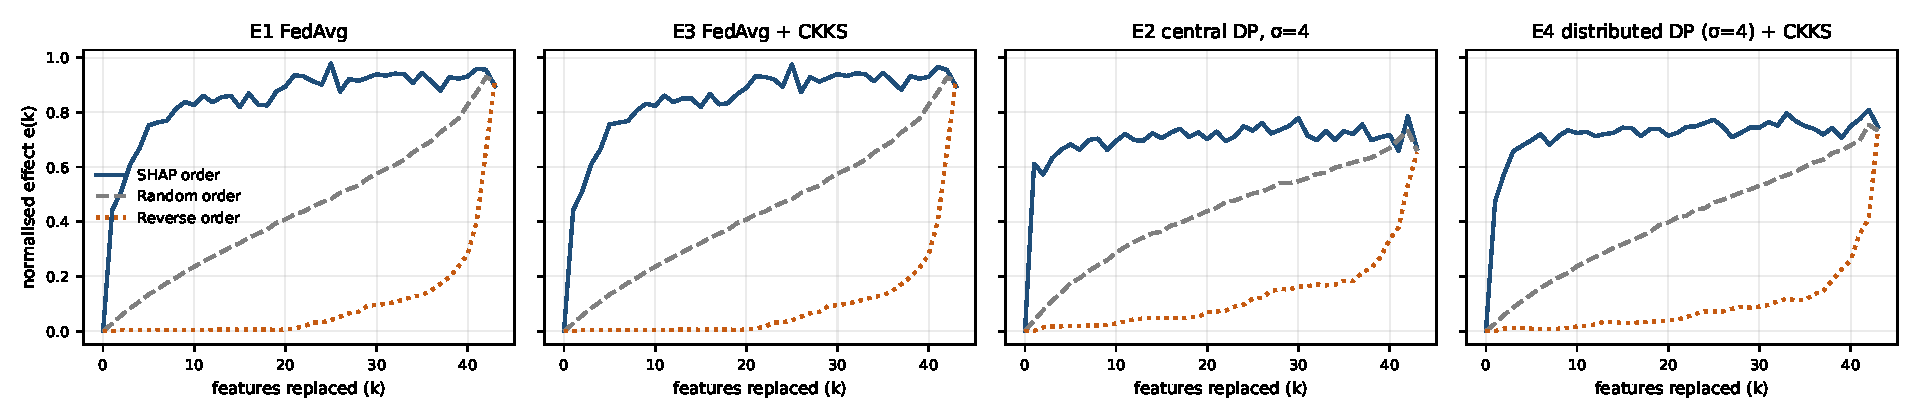
\includegraphics[width=0.95\textwidth]{generated/fig_removal_curves.pdf}
\caption{Removal curves (EARS, conditional replacement): normalised effect $e(k)$ when the first $k$ features are replaced in SHAP order, random order and reverse order, mean over seeds and instances, for E1, E3, E2 ($\sigma=4$) and E4. Source: Authors' own work.}
\label{fig:removal}
\end{figure}

% Generated by experiments/reporting/export_latex.py -- do not edit.
\begin{table}[H]
\centering
\scriptsize
\setlength{\tabcolsep}{3pt}
\caption{Operator cost model by traffic direction (monthly).}
\label{tab:cost}
\begin{tabularx}{\textwidth}{>{\raggedright\arraybackslash}p{3.4cm}*{7}{>{\centering\arraybackslash}X}}
\toprule
Configuration & Upload (GB) & Billable egress (GB) & Egress (USD) & Server compute (USD) & Keys / storage (USD) & Operator total (USD) & Client compute (h) \\
\midrule
E0 Centralised & 1.2 & 0.0 & 0.00 & 0.09 & 0.00 & 0.09 & 0.0 \\
E1 FedAvg & 24.6 & 24.6 & 2.21 & 0.00 & 0.00 & 2.21 & 1.1 \\
E2 central DP ($\sigma{=}4$) & 24.6 & 24.6 & 2.21 & 0.00 & 0.00 & 2.22 & 1.1 \\
E3 CKKS & 504.4 & 24.6 & 2.22 & 0.19 & 1.00 & 3.40 & 2.5 \\
E3 CKKS, shared-mask Top-10\% & 52.5 & 25.4 & 2.29 & 0.02 & 1.00 & 3.31 & 1.3 \\
E4 distributed DP + CKKS & 504.4 & 24.6 & 2.22 & 0.20 & 1.00 & 3.41 & 2.5 \\
\bottomrule
\end{tabularx}
\par\smallskip\raggedright\footnotesize\textit{Source: Authors' own work.} Monthly figures for 30 training jobs and 100 clients (measured 20-client volumes and times scaled by 5). Upload is inbound to the operator and not billed (\$0.00/GB); for E0 it is the raw data transfer. Billable egress: model broadcasts and Top-$k$ masks every job, and the public CKKS context (public key only) once per client per monthly key rotation, at \$0.09/GB. Server compute at \$0.34/h: aggregation and decryption for federated variants, full training for E0. Other: managed key for the wrapped CKKS secret key (\$1/month) or raw-data storage for E0 (\$0.023/GB-month). Client compute is borne by data holders and reported in hours, not dollars. Prices are list-price assumptions; model hosting and inference serving are excluded for all variants.
\end{table}

% Generated by experiments/reporting/export_latex.py -- do not edit.
\begin{table}[H]
\centering
\scriptsize
\setlength{\tabcolsep}{3pt}
\caption{MCDA scores, persona weights, composite scores and rank stability.}
\label{tab:mcda}
\begin{tabularx}{\textwidth}{>{\raggedright\arraybackslash}p{3.4cm}*{9}{>{\centering\arraybackslash}X}}
\toprule
Criterion & E0 & E1 & E2 & E3 & E3 Top-10\% & E4 & W regulated & W retail & W B2B \\
\midrule
C1 Raw data stays local & 1.0 & 5.0 & 5.0 & 5.0 & 5.0 & 5.0 & 0.20 & 0.10 & 0.20 \\
C2 Update confidentiality vs server & 1.0 & 1.0 & 1.0 & 4.0 & 4.0 & 4.0 & 0.20 & 0.05 & 0.20 \\
C3 Formal output privacy & 1.0 & 1.0 & 3.0 & 1.0 & 1.0 & 3.0 & 0.20 & 0.05 & 0.10 \\
C4 Ranking utility & 2.1 & 1.9 & 1.0 & 1.9 & 1.8 & 1.5 & 0.10 & 0.35 & 0.20 \\
C5 Operator cost & 5.0 & 1.5 & 1.5 & 1.0 & 1.0 & 1.0 & 0.05 & 0.20 & 0.10 \\
C6 Explanation fidelity & 4.7 & 5.0 & 1.0 & 5.0 & 5.0 & 2.3 & 0.15 & 0.10 & 0.10 \\
C7 Operational simplicity & 5.0 & 4.0 & 3.0 & 2.0 & 2.0 & 1.0 & 0.10 & 0.15 & 0.10 \\
\midrule Composite &  &  &  &  &  &  &  &  &  \\
\quad Regulated (finance/health) & 2.27 & 2.81 & 2.42 & 3.19 & 3.19 & 3.04 & \multicolumn{3}{l}{} \\
\quad P(rank 1), weights $\pm$ (Dirichlet) & 0.03 & 0.08 & 0.00 & 0.55 & 0.04 & 0.30 & \multicolumn{3}{l}{} \\
\quad Consumer retail & 3.16 & 2.66 & 1.90 & 2.42 & 2.40 & 1.96 & \multicolumn{3}{l}{} \\
\quad P(rank 1), weights $\pm$ (Dirichlet) & 0.86 & 0.10 & 0.00 & 0.04 & 0.00 & 0.00 & \multicolumn{3}{l}{} \\
\quad B2B consortium & 2.39 & 2.73 & 2.25 & 3.08 & 3.07 & 2.83 & \multicolumn{3}{l}{} \\
\quad P(rank 1), weights $\pm$ (Dirichlet) & 0.10 & 0.08 & 0.00 & 0.68 & 0.01 & 0.12 & \multicolumn{3}{l}{} \\
\bottomrule
\end{tabularx}
\par\smallskip\raggedright\footnotesize\textit{Source: Authors' own work.} Scores 1 (worst) to 5 (best). C1, C2, C7 are judgements justified in Table~\ref{tab:mcda_just}; C3--C6 are mapped from measured values (rules in Table~\ref{tab:mcda_just}). P(rank 1): share of 10,000 Dirichlet weight draws centred on the persona (concentration 20) in which the architecture ranks first.
\end{table}

\begin{table}[H]
\centering
\scriptsize
\setlength{\tabcolsep}{3pt}
\caption{Basis of each MCDA criterion score.}
\label{tab:mcda_just}
\begin{tabularx}{\textwidth}{>{\raggedright\arraybackslash}p{3.4cm}>{\raggedright\arraybackslash}X}
\toprule
Criterion & Scoring basis \\
\midrule
C1 Raw data stays local & E0 pools raw interaction records on the server (1). All federated variants keep records on the client and transmit only model updates (5). This criterion describes data flow, not legal compliance. \\
C2 Update confidentiality vs server & E0/E1/E2: the server receives plaintext data or plaintext updates (1; E2 adds noise only after aggregation). E3/E3-TopK/E4: the server receives CKKS ciphertexts and holds no secret key (4, not 5: confidentiality is conditional on RLWE hardness, on the server not colluding with the key holder, and the aggregate is still revealed to the key holder; Top-K additionally reveals the shared coordinate set, which the server chooses). \\
C3 Formal output privacy & Derived from the accountant: 1 without DP; with DP, 5 if epsilon $\leq$ 1, 4 if $\leq$ 3, 3 if $\leq$ 8, 2 otherwise (client-level, delta = 1e-5). \\
C4 Ranking utility & Derived: linear map of risk-adjusted utility, the lower end of the 95\% interval of mean nDCG@10 over seeds, from the random ranking's mean (1) to the pre-cutoff popularity ranking's mean (5). Using the lower bound prevents high between-seed variance under DP noise from scoring as utility. \\
C5 Operator cost & Derived: operator monthly cost mapped on a log scale from the cheapest (5) to the most expensive (1) configuration. \\
C6 Explanation fidelity & Derived: linear map of the SHAP-minus-random removal-curve AUC gap (conditional replacement) from its minimum (1) to its maximum (5). E3 Top-10\% takes E3's value because explanations were not computed for Top-k runs. \\
C7 Operational simplicity & Components to operate beyond plaintext FedAvg: E0 none for federation (5); E1 federation only (4); E2 adds noise calibration and an accountant (3); E3/E3-TopK add key generation, custody and context distribution, and for Top-K a mask protocol (2); E4 adds both (1). \\
\bottomrule
\end{tabularx}
\par\smallskip\raggedright\footnotesize\textit{Source: Authors' own work.} 
\end{table}

\begin{table}[H]
\centering
\scriptsize
\setlength{\tabcolsep}{3pt}
\caption{MCDA sensitivity analysis.}
\label{tab:mcda_sens}
\begin{tabularx}{\textwidth}{>{\raggedright\arraybackslash}p{2.8cm}c>{\raggedright\arraybackslash}p{2.6cm}c>{\raggedright\arraybackslash}X}
\toprule
Persona & Nominal first & Unchanged under $\pm$20\% one-at-a-time? & Mean Kendall $\tau$ (centred) & P(rank 1) under flat Dirichlet weights \\
\midrule
Regulated (finance/health) & E3 & yes & 0.71 & E0 0.41, E3 0.23, E1 0.14, E4 0.14, E3 Top-10\% 0.06, E2 0.02 \\
Consumer retail & E0 & yes & 0.85 & E0 0.41, E3 0.23, E1 0.14, E4 0.14, E3 Top-10\% 0.05, E2 0.02 \\
B2B consortium & E3 & yes & 0.71 & E0 0.42, E3 0.22, E1 0.15, E4 0.14, E3 Top-10\% 0.06, E2 0.02 \\
\bottomrule
\end{tabularx}
\par\smallskip\raggedright\footnotesize\textit{Source: Authors' own work.} One-at-a-time: each weight scaled by 0.8 and 1.2 with renormalisation (14 variants per persona).
\end{table}


\end{document}
